\documentclass[11pt, letterpaper]{article}

% Fonts and Encoding
\usepackage[utf8]{inputenc}
\usepackage[T1]{fontenc}
\usepackage{lmodern} % High-quality Latin Modern vector font

% Math and Symbols
\usepackage{amsmath, amssymb, amsthm, amsfonts, mathrsfs, mathtools}

% Layout and Geometry
\usepackage{geometry}
\geometry{letterpaper, margin=1in}
\setlength{\parindent}{0pt}
\setlength{\parskip}{0.6em}

% Formatting and Graphics
\usepackage{graphicx, xcolor, enumitem, booktabs, array, tabularx}

% TikZ for Illustrations
\usepackage{tikz}
\usetikzlibrary{arrows.meta, positioning, shapes.geometric, calc, backgrounds, matrix}

% Clickable Links and TOC
\usepackage{hyperref}
\hypersetup{
    colorlinks=true,
    linkcolor=blue,
    filecolor=magenta,      
    urlcolor=cyan,
    pdftitle={Comprehensive Problem Set: Laplace Transforms},
}

% Theorem Environments
\newtheorem{theorem}{Theorem}[section]
\newtheorem{lemma}[theorem]{Lemma}
\newtheorem{proposition}[theorem]{Proposition}
\newtheorem{corollary}[theorem]{Corollary}
\theoremstyle{definition}
\newtheorem{definition}{Definition}[section]
\newtheorem{axiom}{Axiom}[section]
\newtheorem{example}{Example}[section]
\theoremstyle{remark}
\newtheorem{remark}{Remark}[section]

% Custom Commands (Enforced standard notation)
\newcommand{\R}{\mathbb{R}}
\newcommand{\N}{\mathbb{N}}
\newcommand{\Z}{\mathbb{Z}}
\newcommand{\Q}{\mathbb{Q}}
\newcommand{\E}{\mathbb{E}}
\newcommand{\Prob}{\mathbb{P}}
\newcommand{\F}{\mathcal{F}}

\title{Comprehensive Problem Set: Laplace Transforms}
\author{Tashfeen Omran}
\date{\today}

\begin{document}

\maketitle
\tableofcontents
\newpage

\section{Concept Checklist \& Question Mapping}

The following table maps the core concepts, problem types, and algebraic tricks derived from the foundational text to the corresponding problems in this document. 

\renewcommand{\arraystretch}{1.5}
\begin{tabularx}{\textwidth}{>{\raggedright\arraybackslash}p{4.5cm} X >{\centering\arraybackslash}p{2.5cm}}
\toprule
\textbf{Concept / Problem Type} & \textbf{Description \& Key Manipulations} & \textbf{Questions} \\ 
\midrule
\textbf{Direct Table \& Linearity} & Distributing the Laplace operator over sums and factoring out constants. & 1, 2, 3 \\ 
\textbf{Algebraic Expansion} & Expanding polynomials (Binomial Theorem) and perfect squares before transforming. & 4, 5, 6, 7 \\ 
\textbf{Trigonometric Identities} & Utilizing power-reducing (half-angle) and product-to-sum formulas for sine and cosine. & 8, 9, 10, 11, 12 \\ 
\textbf{Hyperbolic Functions} & Bypassing memorization by using the exponential definitions of $\sinh(bt)$ and $\cosh(bt)$. & 13, 14 \\ 
\textbf{First Translation Theorem} & The ``s-Shift Cheat'': Handling $e^{at}$ multipliers by shifting $s \to s-a$ at the end. & 15, 16, 17 \\ 
\textbf{Derivative of Transform} & The ``Derivative Sign Toggle'': Handling $t^n$ multipliers via $(-1)^n \frac{d^n}{ds^n} F(s)$. & 18, 19, 20, 21 \\ 
\textbf{Combined Operations} & Sequentially applying shifts and derivatives to complex products. & 22 \\ 
\textbf{Inverse Laplace Transforms} & Mapping from the frequency domain back to time, heavily utilizing Partial Fraction Decomposition. & 23, 24, 25, 26 \\ 
\textbf{Initial Value Problems (IVPs)} & Using $\mathscr{L}\{y'\} = sY(s) - y(0)$ to algebraically solve differential equations. & 27, 28, 29 \\ 
\textbf{Diagnostic Flaws} & Identifying common pitfalls (e.g., False Distribution Trap, incomplete shifting). & 30 \\ 
\bottomrule
\end{tabularx}

\vspace{1em}
\begin{center}
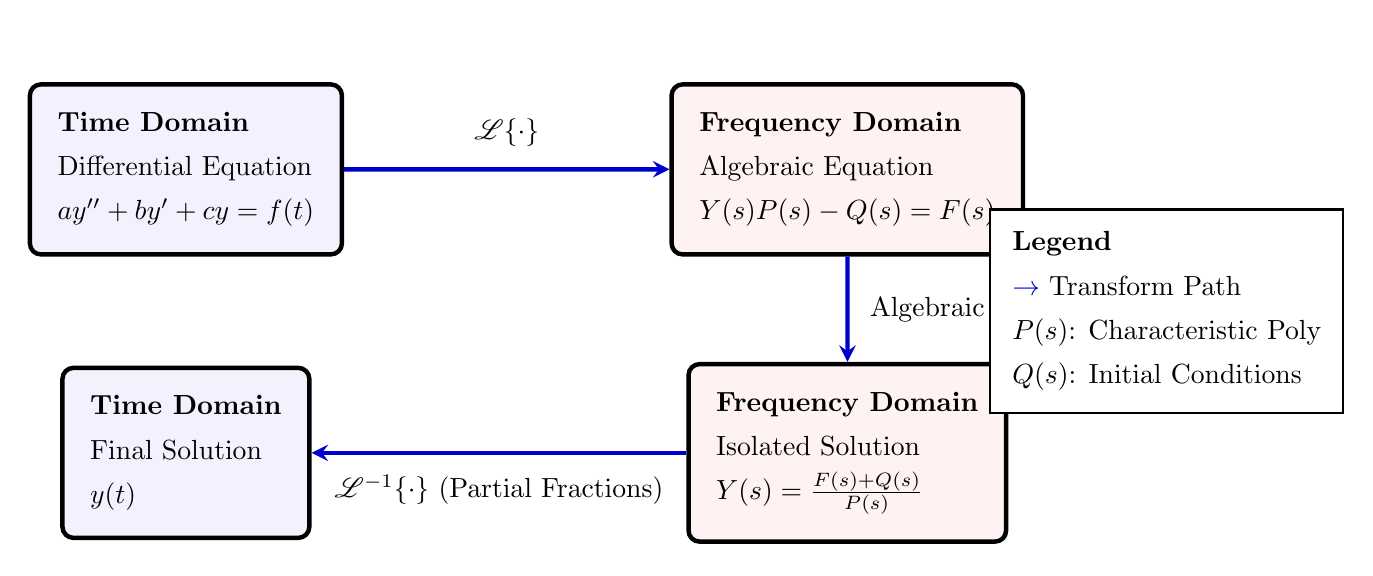
\begin{tikzpicture}[scale=1.2, every node/.style={align=left}]
    % Explicit background fill for cross-compiler safety
    \fill[white] (-1,-1) rectangle (10, 4.5);
    
    % Nodes for IVP Flowchart
    \node[draw, ultra thick, rounded corners, inner sep=10pt, fill=blue!5] (ivp) at (0,3) {\textbf{Time Domain}\\[4pt] Differential Equation\\[4pt] $ay'' + by' + cy = f(t)$};
    \node[draw, ultra thick, rounded corners, inner sep=10pt, fill=red!5] (alg) at (7,3) {\textbf{Frequency Domain}\\[4pt] Algebraic Equation\\[4pt] $Y(s) P(s) - Q(s) = F(s)$};
    \node[draw, ultra thick, rounded corners, inner sep=10pt, fill=red!5] (sol_s) at (7,0) {\textbf{Frequency Domain}\\[4pt] Isolated Solution\\[4pt] $Y(s) = \frac{F(s) + Q(s)}{P(s)}$};
    \node[draw, ultra thick, rounded corners, inner sep=10pt, fill=blue!5] (sol_t) at (0,0) {\textbf{Time Domain}\\[4pt] Final Solution\\[4pt] $y(t)$};
    
    % Arrows
    \draw[->, >=stealth, ultra thick, blue!80!black] (ivp) -- (alg) node[midway, above=4pt, text=black] {$\mathscr{L}\{\cdot\}$};
    \draw[->, >=stealth, ultra thick, blue!80!black] (alg) -- (sol_s) node[midway, right=4pt, text=black] {Algebraic Isolation};
    \draw[->, >=stealth, ultra thick, blue!80!black] (sol_s) -- (sol_t) node[midway, below=4pt, text=black] {$\mathscr{L}^{-1}\{\cdot\}$ (Partial Fractions)};
    
    % Legend using Anchor Pivot Strategy
    \node[draw, thick, fill=white, inner sep=8pt, anchor=west] at (8.5, 1.5) {\textbf{Legend}\\[4pt] \textcolor{blue!80!black}{$\rightarrow$} Transform Path\\[4pt] $P(s)$: Characteristic Poly\\[4pt] $Q(s)$: Initial Conditions};
\end{tikzpicture}
\end{center}

\newpage

\section{Problem Sets}

Evaluate the following Laplace Transforms, Inverse Laplace Transforms, and Initial Value Problems.

\textbf{Direct Table Application \& Linearity}
\begin{enumerate}[label=\textbf{\arabic*.}]
    \item Find $\mathscr{L}\{4t^3 - 2\sin(5t) + 7\}$.
    \item Find $\mathscr{L}\{5e^{-2t} + 3\cos(4t) - t^2\}$.
    \item Find $\mathscr{L}\{\frac{1}{2}t^4 - 3e^{t} + \pi\}$.
\end{enumerate}

\textbf{Algebraic Expansion}
\begin{enumerate}[label=\textbf{\arabic*.}, resume]
    \item Find $\mathscr{L}\{(2t - 1)^2\}$.
    \item Find $\mathscr{L}\{(t^2 + 3)^2\}$.
    \item Find $\mathscr{L}\{(e^{3t} - e^{-3t})^2\}$.
    \item Find $\mathscr{L}\{(t+1)^3\}$.
\end{enumerate}

\textbf{Trigonometric Identities}
\begin{enumerate}[label=\textbf{\arabic*.}, resume]
    \item Find $\mathscr{L}\{\sin^2(3t)\}$.
    \item Find $\mathscr{L}\{\cos^2(2t)\}$.
    \item Find $\mathscr{L}\{\sin(4t)\cos(2t)\}$.
    \item Find $\mathscr{L}\{\cos(5t)\cos(3t)\}$.
    \item Find $\mathscr{L}\{\sin(6t)\sin(t)\}$.
\end{enumerate}

\textbf{Hyperbolic Functions}
\begin{enumerate}[label=\textbf{\arabic*.}, resume]
    \item Find $\mathscr{L}\{\sinh(4t)\}$ using its exponential definition.
    \item Find $\mathscr{L}\{\cosh(2t)\sin(3t)\}$.
\end{enumerate}

\textbf{First Translation Theorem (s-Shift)}
\begin{enumerate}[label=\textbf{\arabic*.}, resume]
    \item Find $\mathscr{L}\{e^{-3t}t^4\}$.
    \item Find $\mathscr{L}\{e^{2t}\cos(5t)\}$.
    \item Find $\mathscr{L}\{e^{-t}\sin^2(t)\}$.
\end{enumerate}

\textbf{Derivative of Transform}
\begin{enumerate}[label=\textbf{\arabic*.}, resume]
    \item Find $\mathscr{L}\{t\sin(2t)\}$.
    \item Find $\mathscr{L}\{t\cos(3t)\}$.
    \item Find $\mathscr{L}\{t^2\sin(t)\}$.
    \item Find $\mathscr{L}\{t^2\cos(2t)\}$.
\end{enumerate}

\textbf{Combined Operational Properties}
\begin{enumerate}[label=\textbf{\arabic*.}, resume]
    \item Find $\mathscr{L}\{t e^{-2t} \sin(3t)\}$.
\end{enumerate}

\textbf{Inverse Laplace Transforms}
\begin{enumerate}[label=\textbf{\arabic*.}, resume]
    \item Find $\mathscr{L}^{-1}\left\{\frac{3}{s^2 + 16}\right\}$.
    \item Find $\mathscr{L}^{-1}\left\{\frac{s - 2}{(s-2)^2 + 9}\right\}$.
    \item Find $\mathscr{L}^{-1}\left\{\frac{4s + 1}{s^2 - s - 6}\right\}$.
    \item Find $\mathscr{L}^{-1}\left\{\frac{2s}{(s^2 + 1)(s-1)}\right\}$.
\end{enumerate}

\textbf{Solving Initial Value Problems (IVPs)}
\begin{enumerate}[label=\textbf{\arabic*.}, resume]
    \item Solve $y' + 4y = e^{-t}$ with $y(0) = 2$.
    \item Solve $y'' + 9y = 0$ with $y(0) = 1$ and $y'(0) = 3$.
    \item Solve $y'' - 3y' + 2y = 4e^{3t}$ with $y(0) = 0$ and $y'(0) = 0$.
\end{enumerate}

\textbf{Diagnostic Testing: "Find the Flaw"}
\begin{enumerate}[label=\textbf{\arabic*.}, resume]
    \item \textbf{Flawed Solution:} $\mathscr{L}\{t^2 e^{3t}\} = \mathscr{L}\{t^2\} \cdot \mathscr{L}\{e^{3t}\} = \frac{2}{s^3} \cdot \frac{1}{s-3} = \frac{2}{s^3(s-3)}$. \\
    \textbf{Your Task:} Identify the conceptual flaw, explain why it is wrong, and provide the correct final answer.
\end{enumerate}

\newpage

\section{Detailed Solutions}

\textbf{Problem 1:} Find $\mathscr{L}\{4t^3 - 2\sin(5t) + 7\}$.
\vspace{0.5em} \\
\textbf{Solution:} By the linearity of the Laplace Transform, we distribute the operator:
\[
\mathscr{L}\{4t^3\} - \mathscr{L}\{2\sin(5t)\} + \mathscr{L}\{7\} = 4\mathscr{L}\{t^3\} - 2\mathscr{L}\{\sin(5t)\} + 7\mathscr{L}\{1\}
\]
Using the standard table formulas $\mathscr{L}\{t^n\} = \frac{n!}{s^{n+1}}$, $\mathscr{L}\{\sin(bt)\} = \frac{b}{s^2+b^2}$, and $\mathscr{L}\{1\} = \frac{1}{s}$:
\begin{align*}
    &= 4\left(\frac{3!}{s^4}\right) - 2\left(\frac{5}{s^2 + 25}\right) + 7\left(\frac{1}{s}\right) \\[4pt]
    &= \frac{24}{s^4} - \frac{10}{s^2 + 25} + \frac{7}{s}
\end{align*}

\vspace{1em}
\textbf{Problem 2:} Find $\mathscr{L}\{5e^{-2t} + 3\cos(4t) - t^2\}$.
\vspace{0.5em} \\
\textbf{Solution:} Apply linearity to separate the terms:
\[
5\mathscr{L}\{e^{-2t}\} + 3\mathscr{L}\{\cos(4t)\} - \mathscr{L}\{t^2\}
\]
Using the standard table values:
\begin{align*}
    &= 5\left(\frac{1}{s + 2}\right) + 3\left(\frac{s}{s^2 + 16}\right) - \frac{2!}{s^3} \\[4pt]
    &= \frac{5}{s + 2} + \frac{3s}{s^2 + 16} - \frac{2}{s^3}
\end{align*}

\vspace{1em}
\textbf{Problem 3:} Find $\mathscr{L}\{\frac{1}{2}t^4 - 3e^{t} + \pi\}$.
\vspace{0.5em} \\
\textbf{Solution:} Apply linearity. Note that $\pi$ is simply a constant.
\[
\frac{1}{2}\mathscr{L}\{t^4\} - 3\mathscr{L}\{e^{t}\} + \pi\mathscr{L}\{1\}
\]
Evaluate each transform:
\begin{align*}
    &= \frac{1}{2}\left(\frac{4!}{s^5}\right) - 3\left(\frac{1}{s - 1}\right) + \pi\left(\frac{1}{s}\right) \\[4pt]
    &= \frac{12}{s^5} - \frac{3}{s - 1} + \frac{\pi}{s}
\end{align*}

\vspace{1em}
\textbf{Problem 4:} Find $\mathscr{L}\{(2t - 1)^2\}$.
\vspace{0.5em} \\
\textbf{Solution:} The Laplace Transform does not distribute over powers. We must first expand the perfect square:
\[
(2t - 1)^2 = 4t^2 - 4t + 1
\]
Now, apply the Laplace Transform to the expanded polynomial:
\begin{align*}
    \mathscr{L}\{4t^2 - 4t + 1\} &= 4\mathscr{L}\{t^2\} - 4\mathscr{L}\{t\} + \mathscr{L}\{1\} \\[4pt]
    &= 4\left(\frac{2}{s^3}\right) - 4\left(\frac{1}{s^2}\right) + \frac{1}{s} \\[4pt]
    &= \frac{8}{s^3} - \frac{4}{s^2} + \frac{1}{s}
\end{align*}

\vspace{1em}
\textbf{Problem 5:} Find $\mathscr{L}\{(t^2 + 3)^2\}$.
\vspace{0.5em} \\
\textbf{Solution:} Expand the perfect square first:
\[
(t^2 + 3)^2 = t^4 + 6t^2 + 9
\]
Apply the Laplace Transform to each term:
\begin{align*}
    \mathscr{L}\{t^4 + 6t^2 + 9\} &= \frac{4!}{s^5} + 6\left(\frac{2!}{s^3}\right) + \frac{9}{s} \\[4pt]
    &= \frac{24}{s^5} + \frac{12}{s^3} + \frac{9}{s}
\end{align*}

\vspace{1em}
\textbf{Problem 6:} Find $\mathscr{L}\{(e^{3t} - e^{-3t})^2\}$.
\vspace{0.5em} \\
\textbf{Solution:} Expand the square. Remember that $e^{3t} \cdot e^{-3t} = e^0 = 1$.
\[
(e^{3t} - e^{-3t})^2 = e^{6t} - 2(e^{3t})(e^{-3t}) + e^{-6t} = e^{6t} - 2 + e^{-6t}
\]
Apply the Laplace Transform:
\begin{align*}
    \mathscr{L}\{e^{6t} - 2 + e^{-6t}\} &= \frac{1}{s - 6} - \frac{2}{s} + \frac{1}{s + 6}
\end{align*}

\vspace{1em}
\textbf{Problem 7:} Find $\mathscr{L}\{(t+1)^3\}$.
\vspace{0.5em} \\
\textbf{Solution:} Expand the polynomial using the Binomial Theorem:
\[
(t+1)^3 = t^3 + 3t^2 + 3t + 1
\]
Apply the Laplace Transform to each term:
\begin{align*}
    \mathscr{L}\{t^3 + 3t^2 + 3t + 1\} &= \frac{3!}{s^4} + 3\left(\frac{2!}{s^3}\right) + 3\left(\frac{1!}{s^2}\right) + \frac{1}{s} \\[4pt]
    &= \frac{6}{s^4} + \frac{6}{s^3} + \frac{3}{s^2} + \frac{1}{s}
\end{align*}

\vspace{1em}
\textbf{Problem 8:} Find $\mathscr{L}\{\sin^2(3t)\}$.
\vspace{0.5em} \\
\textbf{Solution:} We cannot directly transform squared trigonometric functions. We use the power-reducing (half-angle) identity: $\sin^2(\theta) = \frac{1 - \cos(2\theta)}{2}$.
\[
\sin^2(3t) = \frac{1 - \cos(6t)}{2} = \frac{1}{2} - \frac{1}{2}\cos(6t)
\]
Now, apply the Laplace Transform:
\begin{align*}
    \mathscr{L}\left\{\frac{1}{2} - \frac{1}{2}\cos(6t)\right\} &= \frac{1}{2s} - \frac{1}{2}\left(\frac{s}{s^2 + 36}\right) \\[4pt]
    &= \frac{1}{2s} - \frac{s}{2(s^2 + 36)}
\end{align*}

\vspace{1em}
\textbf{Problem 9:} Find $\mathscr{L}\{\cos^2(2t)\}$.
\vspace{0.5em} \\
\textbf{Solution:} Use the power-reducing identity: $\cos^2(\theta) = \frac{1 + \cos(2\theta)}{2}$.
\[
\cos^2(2t) = \frac{1 + \cos(4t)}{2} = \frac{1}{2} + \frac{1}{2}\cos(4t)
\]
Apply the Laplace Transform:
\begin{align*}
    \mathscr{L}\left\{\frac{1}{2} + \frac{1}{2}\cos(4t)\right\} &= \frac{1}{2s} + \frac{1}{2}\left(\frac{s}{s^2 + 16}\right) \\[4pt]
    &= \frac{1}{2s} + \frac{s}{2(s^2 + 16)}
\end{align*}

\vspace{1em}
\textbf{Problem 10:} Find $\mathscr{L}\{\sin(4t)\cos(2t)\}$.
\vspace{0.5em} \\
\textbf{Solution:} Convert the product to a sum using the identity: $\sin(A)\cos(B) = \frac{1}{2}[\sin(A+B) + \sin(A-B)]$.
\[
\sin(4t)\cos(2t) = \frac{1}{2}[\sin(6t) + \sin(2t)]
\]
Apply the Laplace Transform:
\begin{align*}
    \mathscr{L}\left\{\frac{1}{2}\sin(6t) + \frac{1}{2}\sin(2t)\right\} &= \frac{1}{2}\left(\frac{6}{s^2 + 36}\right) + \frac{1}{2}\left(\frac{2}{s^2 + 4}\right) \\[4pt]
    &= \frac{3}{s^2 + 36} + \frac{1}{s^2 + 4}
\end{align*}

\vspace{1em}
\textbf{Problem 11:} Find $\mathscr{L}\{\cos(5t)\cos(3t)\}$.
\vspace{0.5em} \\
\textbf{Solution:} Convert the product to a sum using the identity: $\cos(A)\cos(B) = \frac{1}{2}[\cos(A+B) + \cos(A-B)]$.
\[
\cos(5t)\cos(3t) = \frac{1}{2}[\cos(8t) + \cos(2t)]
\]
Apply the Laplace Transform:
\begin{align*}
    \mathscr{L}\left\{\frac{1}{2}\cos(8t) + \frac{1}{2}\cos(2t)\right\} &= \frac{1}{2}\left(\frac{s}{s^2 + 64}\right) + \frac{1}{2}\left(\frac{s}{s^2 + 4}\right) \\[4pt]
    &= \frac{s}{2(s^2 + 64)} + \frac{s}{2(s^2 + 4)}
\end{align*}

\vspace{1em}
\textbf{Problem 12:} Find $\mathscr{L}\{\sin(6t)\sin(t)\}$.
\vspace{0.5em} \\
\textbf{Solution:} Convert the product to a sum using the identity: $\sin(A)\sin(B) = \frac{1}{2}[\cos(A-B) - \cos(A+B)]$.
\[
\sin(6t)\sin(t) = \frac{1}{2}[\cos(5t) - \cos(7t)]
\]
Apply the Laplace Transform:
\begin{align*}
    \mathscr{L}\left\{\frac{1}{2}\cos(5t) - \frac{1}{2}\cos(7t)\right\} &= \frac{1}{2}\left(\frac{s}{s^2 + 25}\right) - \frac{1}{2}\left(\frac{s}{s^2 + 49}\right) \\[4pt]
    &= \frac{s}{2(s^2 + 25)} - \frac{s}{2(s^2 + 49)}
\end{align*}

\vspace{1em}
\textbf{Problem 13:} Find $\mathscr{L}\{\sinh(4t)\}$ using its exponential definition.
\vspace{0.5em} \\
\textbf{Solution:} The hyperbolic sine function is defined as $\sinh(4t) = \frac{e^{4t} - e^{-4t}}{2}$.
\begin{align*}
    \mathscr{L}\{\sinh(4t)\} &= \frac{1}{2}\mathscr{L}\{e^{4t}\} - \frac{1}{2}\mathscr{L}\{e^{-4t}\} \\[4pt]
    &= \frac{1}{2}\left(\frac{1}{s - 4}\right) - \frac{1}{2}\left(\frac{1}{s + 4}\right)
\end{align*}
Finding a common denominator:
\begin{align*}
    &= \frac{1}{2}\left(\frac{(s + 4) - (s - 4)}{(s - 4)(s + 4)}\right) \\[4pt]
    &= \frac{1}{2}\left(\frac{8}{s^2 - 16}\right) = \frac{4}{s^2 - 16}
\end{align*}

\vspace{1em}
\textbf{Problem 14:} Find $\mathscr{L}\{\cosh(2t)\sin(3t)\}$.
\vspace{0.5em} \\
\textbf{Solution:} Use the exponential definition of $\cosh(2t) = \frac{e^{2t} + e^{-2t}}{2}$.
\[
\cosh(2t)\sin(3t) = \frac{1}{2}e^{2t}\sin(3t) + \frac{1}{2}e^{-2t}\sin(3t)
\]
Apply the First Translation Theorem (s-shift) to each term:
\begin{align*}
    \mathscr{L}\left\{\frac{1}{2}e^{2t}\sin(3t) + \frac{1}{2}e^{-2t}\sin(3t)\right\} &= \frac{1}{2}\mathscr{L}\{\sin(3t)\}\Big|_{s \to s-2} + \frac{1}{2}\mathscr{L}\{\sin(3t)\}\Big|_{s \to s+2} \\[4pt]
    &= \frac{1}{2}\left(\frac{3}{(s - 2)^2 + 9}\right) + \frac{1}{2}\left(\frac{3}{(s + 2)^2 + 9}\right) \\[4pt]
    &= \frac{3}{2((s - 2)^2 + 9)} + \frac{3}{2((s + 2)^2 + 9)}
\end{align*}

\vspace{1em}
\textbf{Problem 15:} Find $\mathscr{L}\{e^{-3t}t^4\}$.
\vspace{0.5em} \\
\textbf{Solution:} By the First Translation Theorem, we find the transform of $t^4$ and shift $s \to s + 3$.
\begin{align*}
    \mathscr{L}\{t^4\} &= \frac{4!}{s^5} = \frac{24}{s^5} \\[4pt]
    \mathscr{L}\{e^{-3t}t^4\} &= \frac{24}{(s + 3)^5}
\end{align*}

\vspace{1em}
\textbf{Problem 16:} Find $\mathscr{L}\{e^{2t}\cos(5t)\}$.
\vspace{0.5em} \\
\textbf{Solution:} Find the transform of $\cos(5t)$ and shift $s \to s - 2$.
\begin{align*}
    \mathscr{L}\{\cos(5t)\} &= \frac{s}{s^2 + 25} \\[4pt]
    \mathscr{L}\{e^{2t}\cos(5t)\} &= \frac{s - 2}{(s - 2)^2 + 25}
\end{align*}

\vspace{1em}
\textbf{Problem 17:} Find $\mathscr{L}\{e^{-t}\sin^2(t)\}$.
\vspace{0.5em} \\
\textbf{Solution:} First, apply the power-reducing identity to $\sin^2(t)$:
\[
e^{-t}\sin^2(t) = e^{-t}\left(\frac{1 - \cos(2t)}{2}\right) = \frac{1}{2}e^{-t} - \frac{1}{2}e^{-t}\cos(2t)
\]
Now apply the Laplace Transform with the appropriate s-shifts ($s \to s + 1$):
\begin{align*}
    \mathscr{L}\left\{\frac{1}{2}e^{-t} - \frac{1}{2}e^{-t}\cos(2t)\right\} &= \frac{1}{2}\left(\frac{1}{s + 1}\right) - \frac{1}{2}\left(\frac{s + 1}{(s + 1)^2 + 4}\right) \\[4pt]
    &= \frac{1}{2(s + 1)} - \frac{s + 1}{2((s + 1)^2 + 4)}
\end{align*}

\vspace{1em}
\textbf{Problem 18:} Find $\mathscr{L}\{t\sin(2t)\}$.
\vspace{0.5em} \\
\textbf{Solution:} Use the derivative property $\mathscr{L}\{tf(t)\} = -\frac{d}{ds}F(s)$.
\begin{align*}
    \mathscr{L}\{\sin(2t)\} &= \frac{2}{s^2 + 4} \\[4pt]
    \mathscr{L}\{t\sin(2t)\} &= -\frac{d}{ds}\left(\frac{2}{s^2 + 4}\right)
\end{align*}
Apply the chain rule (or quotient rule):
\begin{align*}
    -\frac{d}{ds}\left(2(s^2 + 4)^{-1}\right) &= - \left(-2(s^2 + 4)^{-2} \cdot 2s\right) \\[4pt]
    &= \frac{4s}{(s^2 + 4)^2}
\end{align*}

\vspace{1em}
\textbf{Problem 19:} Find $\mathscr{L}\{t\cos(3t)\}$.
\vspace{0.5em} \\
\textbf{Solution:} Use the derivative property.
\begin{align*}
    \mathscr{L}\{\cos(3t)\} &= \frac{s}{s^2 + 9} \\[4pt]
    \mathscr{L}\{t\cos(3t)\} &= -\frac{d}{ds}\left(\frac{s}{s^2 + 9}\right)
\end{align*}
Apply the quotient rule:
\begin{align*}
    -\frac{d}{ds}\left(\frac{s}{s^2 + 9}\right) &= -\left(\frac{1 \cdot (s^2 + 9) - s \cdot (2s)}{(s^2 + 9)^2}\right) \\[4pt]
    &= -\left(\frac{s^2 + 9 - 2s^2}{(s^2 + 9)^2}\right) \\[4pt]
    &= -\left(\frac{9 - s^2}{(s^2 + 9)^2}\right) = \frac{s^2 - 9}{(s^2 + 9)^2}
\end{align*}

\vspace{1em}
\textbf{Problem 20:} Find $\mathscr{L}\{t^2\sin(t)\}$.
\vspace{0.5em} \\
\textbf{Solution:} Multiplying by $t^2$ requires taking the second derivative and multiplying by $(-1)^2 = 1$.
\begin{align*}
    \mathscr{L}\{\sin(t)\} &= \frac{1}{s^2 + 1} \\[4pt]
    \mathscr{L}\{t^2\sin(t)\} &= \frac{d^2}{ds^2}\left(\frac{1}{s^2 + 1}\right)
\end{align*}
First derivative:
\[
\frac{d}{ds}\left((s^2 + 1)^{-1}\right) = -(s^2 + 1)^{-2}(2s) = \frac{-2s}{(s^2 + 1)^2}
\]
Second derivative (using quotient rule):
\begin{align*}
    \frac{d}{ds}\left(\frac{-2s}{(s^2 + 1)^2}\right) &= \frac{-2(s^2 + 1)^2 - (-2s) \cdot 2(s^2 + 1)(2s)}{(s^2 + 1)^4}
\end{align*}
Factor out $(s^2 + 1)$ from the numerator:
\begin{align*}
    &= \frac{(s^2 + 1)[-2(s^2 + 1) + 8s^2]}{(s^2 + 1)^4} \\[4pt]
    &= \frac{-2s^2 - 2 + 8s^2}{(s^2 + 1)^3} \\[4pt]
    &= \frac{6s^2 - 2}{(s^2 + 1)^3}
\end{align*}

\vspace{1em}
\textbf{Problem 21:} Find $\mathscr{L}\{t^2\cos(2t)\}$.
\vspace{0.5em} \\
\textbf{Solution:} Take the second derivative of $F(s) = \frac{s}{s^2 + 4}$.
First derivative (from a similar quotient rule process):
\[
\frac{d}{ds}\left(\frac{s}{s^2 + 4}\right) = \frac{4 - s^2}{(s^2 + 4)^2}
\]
Second derivative (quotient rule):
\begin{align*}
    \frac{d}{ds}\left(\frac{4 - s^2}{(s^2 + 4)^2}\right) &= \frac{-2s(s^2 + 4)^2 - (4 - s^2) \cdot 2(s^2 + 4)(2s)}{(s^2 + 4)^4}
\end{align*}
Factor out $(s^2 + 4)$:
\begin{align*}
    &= \frac{(s^2 + 4)[-2s(s^2 + 4) - 4s(4 - s^2)]}{(s^2 + 4)^4} \\[4pt]
    &= \frac{-2s^3 - 8s - 16s + 4s^3}{(s^2 + 4)^3} \\[4pt]
    &= \frac{2s^3 - 24s}{(s^2 + 4)^3}
\end{align*}

\vspace{1em}
\textbf{Problem 22:} Find $\mathscr{L}\{t e^{-2t} \sin(3t)\}$.
\vspace{0.5em} \\
\textbf{Solution:} This requires a two-step process. We can either shift first then differentiate, or differentiate first then shift. Differentiating first is usually algebraically cleaner.
Step 1: Find $\mathscr{L}\{t\sin(3t)\}$.
\begin{align*}
    \mathscr{L}\{t\sin(3t)\} &= -\frac{d}{ds}\left(\frac{3}{s^2 + 9}\right) \\[4pt]
    &= -\left(\frac{-3(2s)}{(s^2 + 9)^2}\right) = \frac{6s}{(s^2 + 9)^2}
\end{align*}
Step 2: Apply the First Translation Theorem for the $e^{-2t}$ multiplier by shifting $s \to s + 2$.
\begin{align*}
    \mathscr{L}\{e^{-2t} [t\sin(3t)]\} &= \frac{6(s + 2)}{((s + 2)^2 + 9)^2}
\end{align*}

\vspace{1em}
\textbf{Problem 23:} Find $\mathscr{L}^{-1}\left\{\frac{3}{s^2 + 16}\right\}$.
\vspace{0.5em} \\
\textbf{Solution:} This resembles the sine transform $\mathscr{L}\{\sin(bt)\} = \frac{b}{s^2 + b^2}$. Here, $b^2 = 16 \implies b = 4$. We need a $4$ in the numerator.
\begin{align*}
    \mathscr{L}^{-1}\left\{\frac{3}{s^2 + 16}\right\} &= \frac{3}{4}\mathscr{L}^{-1}\left\{\frac{4}{s^2 + 16}\right\} \\[4pt]
    &= \frac{3}{4}\sin(4t)
\end{align*}

\vspace{1em}
\textbf{Problem 24:} Find $\mathscr{L}^{-1}\left\{\frac{s - 2}{(s-2)^2 + 9}\right\}$.
\vspace{0.5em} \\
\textbf{Solution:} This is a shifted cosine transform. The base function is $\frac{s}{s^2 + 9}$, which corresponds to $\cos(3t)$. The shift is $s \to s - 2$, which corresponds to multiplying by $e^{2t}$ in the time domain.
\begin{align*}
    \mathscr{L}^{-1}\left\{\frac{s - 2}{(s-2)^2 + 9}\right\} &= e^{2t}\cos(3t)
\end{align*}

\vspace{1em}
\textbf{Problem 25:} Find $\mathscr{L}^{-1}\left\{\frac{4s + 1}{s^2 - s - 6}\right\}$.
\vspace{0.5em} \\
\textbf{Solution:} Factor the denominator and use Partial Fraction Decomposition.
\[
\frac{4s + 1}{(s - 3)(s + 2)} = \frac{A}{s - 3} + \frac{B}{s + 2}
\]
Multiply by the common denominator:
\[
4s + 1 = A(s + 2) + B(s - 3)
\]
Set $s = 3$: $13 = 5A \implies A = \frac{13}{5}$. \\ \relax
Set $s = -2$: $-7 = -5B \implies B = \frac{7}{5}$.
\begin{align*}
    \mathscr{L}^{-1}\left\{\frac{13/5}{s - 3} + \frac{7/5}{s + 2}\right\} &= \frac{13}{5}e^{3t} + \frac{7}{5}e^{-2t}
\end{align*}

\vspace{1em}
\textbf{Problem 26:} Find $\mathscr{L}^{-1}\left\{\frac{2s}{(s^2 + 1)(s-1)}\right\}$.
\vspace{0.5em} \\
\textbf{Solution:} Use Partial Fraction Decomposition. Since $s^2 + 1$ is an irreducible quadratic, it gets a linear numerator.
\[
\frac{2s}{(s^2 + 1)(s - 1)} = \frac{As + B}{s^2 + 1} + \frac{C}{s - 1}
\]
Multiply by the denominator:
\[
2s = (As + B)(s - 1) + C(s^2 + 1)
\]
Set $s = 1$: $2 = 2C \implies C = 1$. \\ \relax
Set $s = 0$: $0 = -B + C \implies 0 = -B + 1 \implies B = 1$. \\ \relax
Set $s = -1$: $-2 = (-A + 1)(-2) + 1(2) \implies -2 = 2A - 2 + 2 \implies 2A = -2 \implies A = -1$.
\begin{align*}
    \mathscr{L}^{-1}\left\{\frac{-s + 1}{s^2 + 1} + \frac{1}{s - 1}\right\} &= \mathscr{L}^{-1}\left\{-\frac{s}{s^2 + 1} + \frac{1}{s^2 + 1} + \frac{1}{s - 1}\right\} \\[4pt]
    &= -\cos(t) + \sin(t) + e^t
\end{align*}

\vspace{1em}
\textbf{Problem 27:} Solve $y' + 4y = e^{-t}$ with $y(0) = 2$.
\vspace{0.5em} \\
\textbf{Solution:} Take the Laplace Transform of both sides. Let $\mathscr{L}\{y\} = Y(s)$.
\begin{align*}
    (sY(s) - y(0)) + 4Y(s) &= \frac{1}{s + 1} \\[4pt]
    sY(s) - 2 + 4Y(s) &= \frac{1}{s + 1} \\[4pt]
    Y(s)(s + 4) &= 2 + \frac{1}{s + 1} = \frac{2s + 2 + 1}{s + 1} = \frac{2s + 3}{s + 1} \\[4pt]
    Y(s) &= \frac{2s + 3}{(s + 1)(s + 4)}
\end{align*}
Partial fractions:
\[
\frac{2s + 3}{(s + 1)(s + 4)} = \frac{A}{s + 1} + \frac{B}{s + 4} \implies 2s + 3 = A(s + 4) + B(s + 1)
\]
Set $s = -1$: $1 = 3A \implies A = \frac{1}{3}$. \\ \relax
Set $s = -4$: $-5 = -3B \implies B = \frac{5}{3}$.
\begin{align*}
    y(t) &= \mathscr{L}^{-1}\left\{\frac{1/3}{s + 1} + \frac{5/3}{s + 4}\right\} = \frac{1}{3}e^{-t} + \frac{5}{3}e^{-4t}
\end{align*}

\vspace{1em}
\textbf{Problem 28:} Solve $y'' + 9y = 0$ with $y(0) = 1$ and $y'(0) = 3$.
\vspace{0.5em} \\
\textbf{Solution:} Transform the differential equation:
\begin{align*}
    (s^2Y(s) - sy(0) - y'(0)) + 9Y(s) &= 0 \\[4pt]
    s^2Y(s) - s(1) - 3 + 9Y(s) &= 0 \\[4pt]
    Y(s)(s^2 + 9) &= s + 3 \\[4pt]
    Y(s) &= \frac{s + 3}{s^2 + 9} = \frac{s}{s^2 + 9} + \frac{3}{s^2 + 9}
\end{align*}
Take the inverse transform:
\begin{align*}
    y(t) &= \cos(3t) + \sin(3t)
\end{align*}

\vspace{1em}
\textbf{Problem 29:} Solve $y'' - 3y' + 2y = 4e^{3t}$ with $y(0) = 0$ and $y'(0) = 0$.
\vspace{0.5em} \\
\textbf{Solution:} Transform the equation (initial conditions are zero, so derivatives simplify):
\begin{align*}
    s^2Y(s) - 3sY(s) + 2Y(s) &= \frac{4}{s - 3} \\[4pt]
    Y(s)(s^2 - 3s + 2) &= \frac{4}{s - 3} \\[4pt]
    Y(s)(s - 1)(s - 2) &= \frac{4}{s - 3} \\[4pt]
    Y(s) &= \frac{4}{(s - 1)(s - 2)(s - 3)}
\end{align*}
Partial fractions:
\[
\frac{4}{(s - 1)(s - 2)(s - 3)} = \frac{A}{s - 1} + \frac{B}{s - 2} + \frac{C}{s - 3}
\]
\[
4 = A(s - 2)(s - 3) + B(s - 1)(s - 3) + C(s - 1)(s - 2)
\]
Set $s = 1$: $4 = A(-1)(-2) \implies 2A = 4 \implies A = 2$. \\ \relax
Set $s = 2$: $4 = B(1)(-1) \implies -B = 4 \implies B = -4$. \\ \relax
Set $s = 3$: $4 = C(2)(1) \implies 2C = 4 \implies C = 2$.
\begin{align*}
    y(t) &= \mathscr{L}^{-1}\left\{\frac{2}{s - 1} - \frac{4}{s - 2} + \frac{2}{s - 3}\right\} \\[4pt]
    &= 2e^t - 4e^{2t} + 2e^{3t}
\end{align*}

\vspace{1em}
\textbf{Problem 30:} \textbf{Flawed Solution:} $\mathscr{L}\{t^2 e^{3t}\} = \mathscr{L}\{t^2\} \cdot \mathscr{L}\{e^{3t}\} = \frac{2}{s^3} \cdot \frac{1}{s-3} = \frac{2}{s^3(s-3)}$. \\
\textbf{Your Task:} Identify the conceptual flaw, explain why it is wrong, and provide the correct final answer.
\vspace{0.5em} \\
\textbf{Solution:} 
\textbf{Flaw:} The student fell into the \textit{False Distribution Trap}. The Laplace Transform of a product is \textbf{not} the product of their individual Laplace Transforms (multiplication in time corresponds to convolution in frequency). \\ \relax
\textbf{Correct Method:} We must use the First Translation Theorem (s-shift). We find the transform of the base function $t^2$ and shift every instance of $s$ by $(s - 3)$.
\begin{align*}
    \mathscr{L}\{t^2\} &= \frac{2}{s^3} \\[4pt]
    \mathscr{L}\{e^{3t}t^2\} &= \frac{2}{(s - 3)^3}
\end{align*}

\end{document}